\documentclass[12pt,letterpaper]{article}

\usepackage{titlepic}

\usepackage[utf8]{inputenc}

\usepackage{amsmath}

\usepackage{amsfonts}

\usepackage{amssymb}

\usepackage{graphicx}

\usepackage[left=1in,right=1in,top=1in,bottom=1in]{geometry}

\usepackage{hyperref}

\usepackage{float}

\usepackage{setspace}

\author{Jonathan Zhou}

\title{Pictionary over Local Area Networks in the Java Language\footnote{Code: \url{https://drive.google.com/open?id=1hjIwU4qBRfIKhUcc5MUmuA5sfffzNF0B}}}



\begin{document}
\maketitle

\begin{figure}[H]
\centering
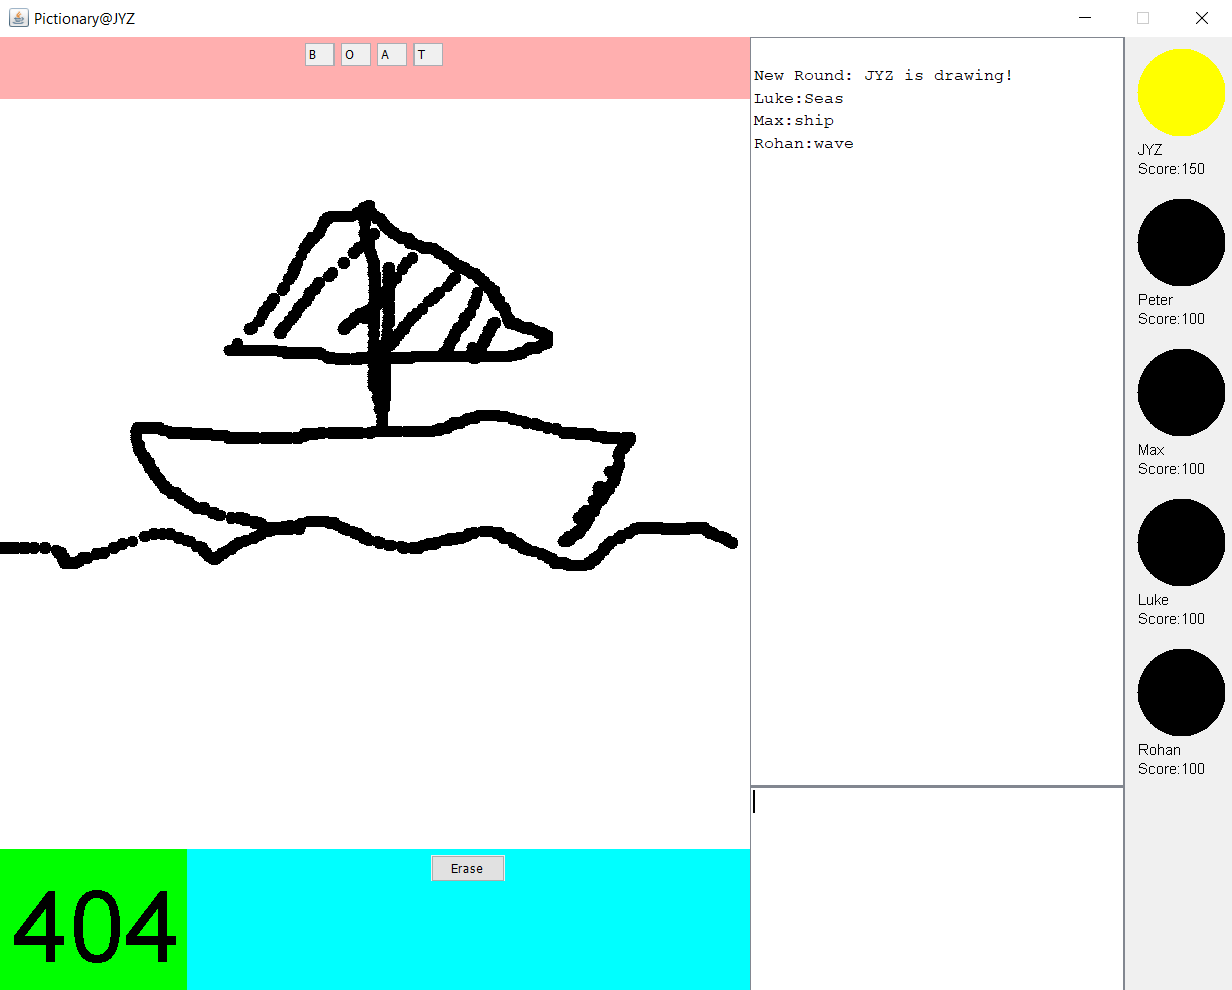
\includegraphics[width=5in]{sampleGameplay.PNG}

\caption{Sample Gameplay in Pictionary over LAN}
\end{figure}
\thispagestyle{empty}

\newpage

\doublespacing

\section*{Product Description}

\textit{Pictionary over LAN} provides a variant of Pictionary which works over networks. It follows a multiple-client server architecture. Client connections are made via the invocation of a Pictionary client GUIs, where a bidirectional communication channel will be established where the client and server concurrently pass messages to communicate game data (e.g. drawing, new round, hint, guess).

The game commences once all players join. The server loops through all game rounds and players such that all players have a chance to draw once for each round. All guessers have until time runs out to guess the drawer's word. Points are awarded based on speed. Players can see previously made incorrect guesses from other players via a chat interface. A round terminates upon either the exhaustion of time, or if all players have guessed correctly. The player with the most points at the end is the winner.

The goal of this game is to provide a fun experience which is simple, easy to distribute, multiplayer, and runs on many different devices. The game fosters social interaction and enables leisure time to be spent between friend and stranger alike without worry about configuration details.

\textit{Pictionary over LAN} offers advantages in convenience, openness, and privacy compared to the popular online game \textit{skribbl.io} and a traditional, pen and paper style of Pictionary. \textit{Pictionary over LAN} gives users the ability to host and configure their own server. As game is intended to work over LAN, firewalls don't interfere with game operation. However, the game can also be run across other network architectures. The game offers much in terms of flexibility, e.g. custom vocabulary banks. On the other hand, \textit{skribbl.io}, which exposes players to the internet and constant connectivity, has advertisements and other superfluous UI elements, contends with web-browser overheads, and has public games marred by inappropriate content. Though the creation of private parties is supported, data is still proxied over the wider internet. The spartan design of \textit{Pictionary over LAN} is an intentional advantage.

With the increased proliferation of digital devices and a decline in the use of pen in paper \textit{Pictionary over LAN} offers much in terms of convenience over traditional Pictionary. Large quantities of wastepaper and set up of a physical space is eliminated. \textit{Pictionary over LAN} eliminates the need for players to serve as a moderators and tabulators for a game. Using a digital human input device to draw figures also provides a novel challenge.


\section*{Market Analysis}

\textit{Pictionary over LAN} is intended for people ages 10 and up. Players must sociable, capable of understanding vocabulary, and have fine motor control. As the game offers Unicode support, the word bank is customizable, and usage doesn’t require an understanding of the English language beyond a few keywords, the game is readily localizable. Network parameters only need be understood at a superficial level. Although configuring and instantiating a server is slightly more difficult than joining as a client, this process is still very simple. 

There is precedence for games such as \textit{Pictionary over LAN} within the wider game area, as evident in the success of \textit{skribbl.io} and \textit{Quick, Draw!}. This success extends beyond the browser with many desktop games supporting multiplayer connectivity over LAN.

The server and client would be distributed in both binary and source forms, bundled as one package. The software may be run portably for convenience. Distributions of this software can either be obtained online or from other players where the binaries may simply be copied. This allows for the game to be proliferated even when an internet connection is not available.  Due to the nature of the market (where many similarly free alternatives already available), it would be essentially impossible to monetize this product and thus it would be offered free of charge. However, this is not to say that such software has no value as the proliferation of such serves to create various forms of non-monetary benefits through the enjoyment of the game, education (through vocabulary acquisition) and the creation and fostering of new social bonds.

\end{document}